\section{Exact NNI Refinement}
\subsection{A local structural-entropy identity}
For disjoint sets $X,Y$, write
$W(X,Y)=\sum_{u\in X,v\in Y}w_{uv}$. Consider the rotation shown in
Fig.~\ref{fig:nni}. Let $X=A\cup B$, $Y=B\cup C$, and
$P=A\cup B\cup C$.

\begin{figure}[t]
\centering
\begin{tikzpicture}[
  level distance=8mm,
  every node/.style={font=\small},
  internal/.style={circle,draw=black!55,fill=black!5,inner sep=1.7pt,
                   line width=0.55pt},
  module/.style={rounded corners=2pt,draw=black!55,minimum width=9mm,
                 minimum height=5.5mm,line width=0.55pt},
  edge from parent/.style={draw=black!65,-,line width=0.65pt}
]
\node[internal] (p1) at (0,0) {$P$};
\node[internal] (x) at (-0.7,-0.8) {$X$};
\node[module,fill=blue!12] (c1) at (0.7,-0.8) {$C$};
\node[module,fill=cyan!13] (a1) at (-1.1,-1.65) {$A$};
\node[module,fill=orange!18] (b1) at (-0.3,-1.65) {$B$};
\draw (p1)--(x) (p1)--(c1) (x)--(a1) (x)--(b1);
\node[text=red!75!black,font=\small\bfseries] at (2.0,-0.72)
  {$\xrightarrow{\quad\mathrm{exact\ NNI}\quad}$};
\node[text=black!60,font=\scriptsize] at (-0.7,-2.05) {$X=A\cup B$};
\node[internal] (p2) at (4,0) {$P$};
\node[module,fill=cyan!13] (a2) at (3.3,-0.8) {$A$};
\node[internal] (y) at (4.7,-0.8) {$Y$};
\node[module,fill=orange!18] (b2) at (4.3,-1.65) {$B$};
\node[module,fill=blue!12] (c2) at (5.1,-1.65) {$C$};
\draw (p2)--(a2) (p2)--(y) (y)--(b2) (y)--(c2);
\node[text=black!60,font=\scriptsize] at (4.7,-2.05) {$Y=B\cup C$};
\node[rounded corners=2pt,draw=blue!35,fill=blue!4,
      minimum width=7.7cm,minimum height=5.5mm,font=\scriptsize]
  at (2.0,-2.55)
  {three volumes $V_X,V_Y,V_P$ + two cross weights $W(A,B),W(B,C)$
   $\Longrightarrow$ verified $\Delta H^T$};
\end{tikzpicture}
\caption{A rooted NNI replaces only $X=A\cup B$ by $Y=B\cup C$. The
highlighted local statistics determine the exact full-objective change; all
leaves and the surrounding tree remain fixed.}
\label{fig:nni}
\end{figure}

\begin{theorem}[Exact weighted NNI delta]\label{thm:delta}
For an eligible rotation with $V_X,V_Y,V_P>0$, the change in tree structural
entropy is
\begin{equation}
 \Delta \HT=
 \frac{2}{\vol(V)}\left[
 W(A,B)\log_2\frac{V_P}{V_X}+
 W(B,C)\log_2\frac{V_Y}{V_P}
 \right].
 \label{eq:nni-delta}
\end{equation}
The symmetric alternative follows by exchanging $A$ and $B$.
\end{theorem}

Equivalently, the bracket in Eq.~\eqref{eq:nni-delta} is
\begin{equation}
 W(B,C)\log_2 V_Y-W(A,B)\log_2 V_X
 +\bigl(W(A,B)-W(B,C)\bigr)\log_2 V_P.
 \label{eq:nni-expanded}
\end{equation}
The parent-volume term in Eq.~\eqref{eq:nni-expanded} is essential and cannot
be dropped merely because the edit is local.

\begin{proof}
First suppose the three child modules have positive volume; the zero-volume
boundary case follows by deleting modules with no incident positive-weight
edge and taking the corresponding zero-contribution limit.
Only the terms for $A,B,C,X$, and $Y$ can change. Omitting the common factor
$1/\vol(V)$, their old and new contributions are
\begin{align*}
 L_{\rm old}={}&g_A\log_2\frac{V_X}{V_A}
 +g_B\log_2\frac{V_X}{V_B}
 +g_X\log_2\frac{V_P}{V_X}
 +g_C\log_2\frac{V_P}{V_C},\\
 L_{\rm new}={}&g_A\log_2\frac{V_P}{V_A}
 +g_B\log_2\frac{V_Y}{V_B}
 +g_C\log_2\frac{V_Y}{V_C}
 +g_Y\log_2\frac{V_P}{V_Y}.
\end{align*}
Use $g_X=g_A+g_B-2W(A,B)$ and
$g_Y=g_B+g_C-2W(B,C)$. In $L_{\rm new}-L_{\rm old}$, the coefficients of
$g_A,g_B,g_C$ telescope to zero. The remaining terms are
\[
 2W(A,B)\log_2(V_P/V_X)+2W(B,C)\log_2(V_Y/V_P).
\]
Restoring $1/\vol(V)$ proves Eq.~\eqref{eq:nni-delta}. In particular, external boundary
weights and $W(A,C)$ do not enter the rotation delta.
\end{proof}

Equation~\eqref{eq:nni-delta} is evaluated from cached descendant sets and the
sparse adjacency lists. Every selected move is also checked by rebuilding all
module volumes and cuts and recomputing Eq.~\eqref{eq:tree-se}. This second path
is slower but makes a formula or tree-edit error observable rather than silent.

\subsection{One-step certificate and compound escape}
\begin{algorithm}[H]
\caption{Exact NNI refinement of one candidate tree}\label{alg:nni}
\KwIn{Graph $G$, tree $T$, tolerance $\varepsilon$, barrier $\beta$, beam $b$}
\Repeat{no improving one-step move exists}{
  evaluate Eq.~\eqref{eq:nni-delta} for every legal NNI of $T$\;
  apply the most negative move and verify the full objective\;
}
\For{at most $R$ compound rounds}{
  retain the $b$ first moves with smallest $\Delta H$ and $\Delta H\le\beta$\;
  expand every legal second NNI from each retained intermediate tree\;
  \If{no two-move endpoint has entropy below $H^T(G)$}{break\;}
  commit the best endpoint; rerun one-step descent\;
}
\Return{$T$}
\end{algorithm}

\begin{proposition}[Monotonicity and local certificate]\label{prop:local}
One-step refinement never increases $\HT(G)$. If it stops before its move
budget, the returned tree has no improving rooted NNI on any eligible binary
parent--child edge.
\end{proposition}
\begin{proof}
Only moves with $\Delta\HT<-\varepsilon$ are committed, and their endpoint is
independently verified. At termination every enumerated legal move has
$\Delta\HT\ge-\varepsilon$.
\end{proof}

Strict one-step descent can stop before a better tree separated by a shallow
barrier. Algorithm~\ref{alg:nni} therefore keeps a bounded beam of first moves
whose increase is at most $\beta$ and evaluates a second NNI. It never commits
the intermediate tree alone.

\begin{proposition}[Safe compound search]\label{prop:compound}
The compound stage never worsens its input. It can reach an improving endpoint
even when every one-step neighbor is non-improving.
\end{proposition}
\begin{proof}
A pair is committed only after the final tree is fully recomputed and found to
have lower entropy than the tree preceding the pair. The first move is not
committed independently, so its sign cannot weaken the output guarantee. A
two-edge path in tree space may have a positive first delta and a negative net
delta; the regression witness in Sec.~\ref{sec:experiments} instantiates this
case.
\end{proof}

\subsection{Fast multi-start SE--NNI}
\SEAlg applies Algorithm~\ref{alg:nni} independently to SE-agglomerative,
recursive-SE, and Paris starts and returns the candidate with minimum verified
entropy. This replaces the generic collapse/relocation stage of
\texttt{se\_hier}. The initializer is recorded for every output, so gains can
be attributed either to construction or refinement. With $n$ leaves there are
at most $2(n-2)$ oriented NNI alternatives per sweep, versus a substantially
larger generic space of source--destination tree edits. Our implementation
uses best improvement, cached leaf sets, sparse cross-weight scans, and an
$O(m\log h+n)$ full verification only for a selected move, where $h$ is tree
height. We make runtime claims empirically rather than assuming balanced trees.
